% =============================================================================
% File:  MATLAB2.tex -- 
% Author(s): Valentin Plugaru (valentin.plugaru@uni.lu)
% Time-stamp: <Tue 2015-06-16 09:22 svarrette>
% 
% Copyright (c) 2015 Valentin Plugaru<Valentin.Plugaru@uni.lu>
% 
% For more information:
% - LaTeX: http://www.latex-project.org/
% - Beamer: https://bitbucket.org/rivanvx/beamer/
% - LaTeX symbol list:
% http://www.ctan.org/tex-archive/info/symbols/comprehensive/symbols-a4.pdf
% =============================================================================

\documentclass{beamer}
% \documentclass[draft]{beamer}
\usepackage{_style}
\newcommand{\cmdlinegaia}[1]{\promptline{(gaia)}{#1}}
\newcommand{\cmdlinechaos}[1]{\promptline{(chaos)}{#1}}
\newcommand{\cmdlinefrontend}[1]{\promptline{(frontend)}{#1}}
\newcommand{\cmdlinenode}[1]{\promptline{(node)}{#1}}
\newcommand{\cmdlinecomment}[1]{\hfill{\tiny \textcolor{red}{\textit{\# #1}}}}
\newcommand{\ULHPC}{\href{http://hpc.uni.lu}{UL HPC Platform}\xspace}


% The key part to use my theme -- if you precise nothing, the image that
% illustrate the slides is assumed to be images/slides_image.jpg
\usetheme[image=images/logo_hpc-shool2015.pdf]{Falkor}

% Not integrated in my theme as not everybody wants that
\AtBeginSection[]
{
  \frame{
    \frametitle{Summary}
    {\scriptsize\tableofcontents[currentsection]}
  }
}

\graphicspath{{images/}} % Add this directory to the searched paths for graphics


%%%%%%%%%% Header %%%%%%%%%%%%
\title{MATLAB on UL HPC}
\subtitle{Checkpointing \& parallel execution}

\author{Valentin Plugaru}
\institute[UL HPC, PCOG Research unit]{
  \href{http://hpc.uni.lu}{UL HPC} Management Team,\\
  Parallel Computing and Optimization Group (\href{http://pcog.uni.lu}{PCOG}),
  University of Luxembourg (\href{http://www.uni.lu}{UL}), Luxembourg
}

% Mandatory to **declare** a logo to be placed on the bottom right -- normally the
% university logo. ADAPT ACCORDINGLY:
\pgfdeclareimage[height=0.8cm]{logo}{images/logo_UL.pdf}

\date{}

%%%%%%%%%%%%% Body %%%%%%%%%%%%%%%
\begin{document}

\begin{frame}
  \vspace{2.5em}
  \titlepage
\end{frame}

\begin{frame}
  \begin{center}
      \textbf{Latest versions available on
        \href{https://github.com/ULHPC/}{Github}}:
      \vfill
      \begin{description}
        \item[UL HPC tutorials:] \hfill
          \myurl{https://github.com/ULHPC/tutorials}
        \item[UL HPC School:] \hfill
          \myurl{https://hpc.uni.lu/hpc-school}
        \item[This tutorial's sources:] \hfill
          \myurl{https://github.com/ULHPC/tutorials/tree/devel/advanced/MATLAB2}
      \end{description}
  \end{center}
\end{frame}

% ......
\frame{
  \frametitle{Summary}
  {\scriptsize
    \tableofcontents
  }
}

\section{Pre-requisites}

% .......
\begin{frame}[fragile]
\frametitle{Tutorial files}
  Sample MATLAB scripts used in the tutorial\\
  \begin{itemize}
   \item download only the scripts: \\
  \begin{cmdline}
    \cmdlinefrontend{mkdir \$HOME/matlab-tutorial2} \\
    \cmdlinefrontend{cd \$HOME/matlab-tutorial2} \\
    \cmdlinefrontend{wget \myurl{https://raw.github.com/ULHPC/tutorials/devel/advanced/MATLAB2/code/example1.m}} \\
    \cmdlinefrontend{wget \myurl{https://raw.github.com/ULHPC/tutorials/devel/advanced/MATLAB2/code/example2.m}} \\
    \cmdlinefrontend{wget \myurl{https://raw.github.com/ULHPC/tutorials/devel/advanced/MATLAB2/code/yahoo\_finance\_data.m}} \\
  \end{cmdline}
  \item \textit{or} download the full repository and link to the MATLAB tutorial: \\
  \begin{cmdline}
    \cmdlinefrontend{git clone \myurl{https://github.com/ULHPC/tutorials.git}} \\
    \cmdlinefrontend{ln -s tutorials/advanced/MATLAB2/ \$HOME/matlab-tutorial2} \\
  \end{cmdline}  
  \end{itemize}

\end{frame}

\begin{frame}[fragile]
\frametitle{X Window System}
  In order to see locally the MATLAB graphical interface, \\
  a package providing the X Window System is required:
  \begin{itemize}
    \item on OS X: \textbf{XQuartz} \hfill\myurl{http://xquartz.macosforge.org/landing/}
    \item on Windows: \textbf{VcXsrv} \hfill\myurl{http://sourceforge.net/projects/vcxsrv/}
  \end{itemize}
  \hfill \\ \hfill \\ %\hfill \\
  
  Now you will be able to connect with X11 forwarding enabled:
  \begin{itemize}
    \item on Linux \& OS X: \\
    \begin{cmdline}
       \cmdlineentry{ssh access-gaia.uni.lu} \textbf{-X}
    \end{cmdline}
    \item on Windows, with Putty \\
     Connection $\rightarrow$ SSH $\rightarrow$ X11 $\rightarrow$ \textbf{Enable X11 forwarding}
  \end{itemize}  
\end{frame}

% ===============================================
\section{Objectives}

% ............
\begin{frame}
  \frametitle{Objectives of this PS}

  Better understand the usage of MATLAB on the \ULHPC
 
  \begin{exampleblock}{}
    \begin{itemize}
      \item application-level checkpointing
      \begin{itemize}
        \item using in-built MATLAB functions
      \end{itemize}
     \end{itemize}
   \end{exampleblock}
   \pause
   \begin{exampleblock}{}
    \begin{itemize}
     \item taking advantage of some parallelization capabilities
      \begin{itemize}
       \item use of \textbf{parfor}
       \item use of GPU-enabled functions
      \end{itemize}
     \end{itemize}
    \end{exampleblock}   
    \pause
    \begin{exampleblock}{}
    \begin{itemize}
     \item adapting the parallel code with checkpoint/restart features
    \end{itemize}
    \end{exampleblock}   

\end{frame}

\section{Checkpointing}

\begin{frame}
  \frametitle{Checkpointing}
 
  \begin{block}{What is it?}
  Technique for adding fault tolerance to your application. \\ 
  You adapt your code to (regularly) save a snapshot of the environment (workspace), and restart execution from the snapshot in case of failure.
  \end{block}
   \pause
   \begin{block}{Why make the effort to checkpoint?}
    \begin{itemize}
     \item because your code may take longer to execute than the maximum walltime allowed
     \item because losing (precious) hours or days of computation \emph{when} something fails may (should!) not be acceptable
     \end{itemize}
    \end{block}   
\end{frame}


\begin{frame}
  \frametitle{Checkpointing pitfalls}
  \begin{alertblock}{}
    \begin{itemize}
     \item checkpointing (too) often can be counterproductive
     \begin{itemize}
      \item saving state in each loop may take longer than its actual computing time
      \item saving state incrementally can lead to fast exhaustion of your \$HOME space
      \item in extreme cases can lead to platform instability -- especially if running parallel jobs!
     \end{itemize}
   \end{itemize}
   \end{alertblock}   
   \pause
   \begin{alertblock}{}
    \begin{itemize}
     \item checkpointing (especially parallel) code can be tricky
     \item extra-care required if checkpointing simulations involving RNG (e.g. Monte Carlo-based experiments)
     \item ensure results consistency after you add checkpointing
     \end{itemize}
   \end{alertblock}   
\end{frame}


\begin{frame}
  \frametitle{Checkpointing basics}
    \begin{enumerate}
     \item Check that a checkpoint file exists: \hfill {\tiny \texttt{exist('save.mat','file')}}
     \item If it exists, restore workspace data from it:\hfill {\tiny \texttt{load('save.mat')}}
     \pause
     \item During computing steps, use control variables to direct (re)start of computation
     \pause
     \item Every $n$ loops, or if execution time (in loop or since startup) is above threshold, checkpoint:
     \begin{itemize}
      \item save full workspace state:\hfill {\tiny \texttt{save('save.tmp')}}
      \item save partial state:\hfill {\tiny \texttt{save('save.tmp', 'var1', 'var2')}}
     \end{itemize}
     \pause
     \item Rename state file to final name:\hfill {\tiny \texttt{system('mv save.tmp save.mat')}}
     \begin{itemize}
      \item this process ensures that in case of failure during checkpointing, next execution doesn't try to restart from incomplete state
     \end{itemize}  
   \end{enumerate}
\end{frame}

\begin{frame}
  \frametitle{When to trigger checkpointing?}

    \begin{itemize}
     \item when (loop) execution time is above threshold (e.g. 1h):
     \begin{itemize}
      \item use \texttt{tic} and \texttt{toc} stopwatch functions, remember they can be assigned to variables
      \item use the \texttt{clock} function
      \item add some \emph{randomness} to the threshold if you run several instances in parallel!
     \end{itemize}
     \pause
     \vspace{3ex}
     \item every $n$ loop executions
     \begin{itemize}
      \item remember that saving state takes time, depending on workspace size \& shared filesystem usage, and
      \item if loops finish fast your code may be slowed down considerably
      \item add some \emph{randomness} to $n$ if you run several instances in parallel!
     \end{itemize}  
   \end{itemize}
\end{frame}


\subsection{Example 1 revisited}

% .......
\frame{
  \frametitle{Adding checkpointing to seq. code}
  \textbf{example1.m}: non-interactive script that shows:
\begin{itemize}
 \item the use of a stopwatch timer
 \item how to use an external function (financial data retrieval)
 \item how to use different plotting methods
 \item how to export the plots in different graphic formats
\end{itemize} 

\begin{block}{Tasks to tackle with checkpointing}
   \begin{itemize}
    \item modify the script to download data for Fortune100 companies
    \item add \& test checkpointing to save state after each company's data is downloaded
    \item more granular downloads - modify download period from 1 year to 1 month, add \& test checkpointing to save state after each download
   \end{itemize}
\vspace{-2ex}
\end{block}
}

\section{Parallelization}

\begin{frame}
  \frametitle{Reference documentation}
  \begin{itemize}
   \item \emph{Parallel Computing Toolbox} \hfill\myurl{http://www.mathworks.nl/help/distcomp/index.html}
   \item Parallel for-Loops (parfor) \hfill\myurl{http://www.mathworks.nl/help/distcomp/getting-started-with-parfor.html}
   \item GPU Computing \hfill\myurl{http://www.mathworks.nl/discovery/matlab-gpu.html}
  \end{itemize}
\end{frame}

\begin{frame}
  \frametitle{Accelerate the time to result}
  \begin{itemize}
   \setlength\itemsep{3ex}
   \item[Option 1:] Split input over several parallel, independent, MATLAB jobs
   \begin{itemize}
    \item great \emph{if} it's possible (embarrassingly parallel problem)
   \end{itemize}
   \pause
   \item[Option 2:] Use \emph{parfor} to execute loop iterations in parallel
   \begin{itemize}
    \item single node \emph{only}
    \item we have 120 \& 160 core nodes on which big problems can be tackled
   \end{itemize}
   \pause
   \item[Option 3:] Use GPU-enabled functions that work on the \emph{gpuArray} data type
   \begin{itemize}
    \item \emph{require} the code to be run on GPU nodes (subset of Gaia)
    \item \emph{great speedup} for some workloads
    \item \emph{295} in-built MATLAB functions work on gpuArray \\ { \tiny including discrete Fourier transform, matrix multiplication, left matrix division}
   \end{itemize}
   \pause
   \item[Option 4:] MATLAB Distributed Computing Server (MDCS)
   \begin{itemize}
    \item allows multi-node parallel execution
    \item \emph{not yet} part of the UL MATLAB license
   \end{itemize}
   \end{itemize}
\end{frame}


\subsection{Example 2 revisited}

% .......
\frame{
  \frametitle{Speed up your seq. code}
 
  \textbf{example2.m}: non-interactive script that shows:
  \begin{itemize}
   \item the serial execution of time consuming operations
   \begin{itemize}
    \item the parallel execution and relative speedup vs serial execution
    \item setting the \# of parallel threads through environment variables
    \item GPU-based parallel execution
    \end{itemize}
  \end{itemize}
  \only<1>{\centering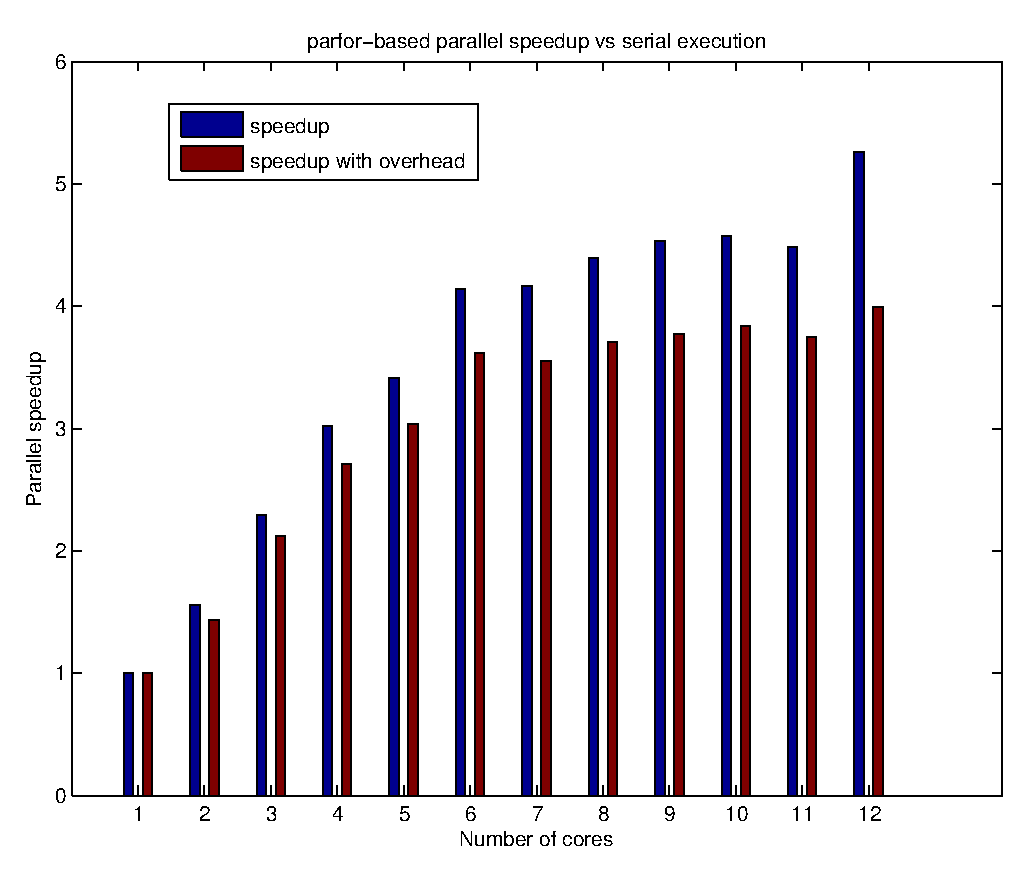
\includegraphics[width=0.45\linewidth,keepaspectratio]{plots/parfor-speedup.eps}}
  \only<2>{\begin{block}{Tasks to tackle}
   \begin{itemize}
    \item execute the script on regular vs GPU nodes (with different GPUs)
    \item increase \# of iterations, matrix size
    \item increase \# of workers with/without changing the \# of requested cores
    \item modify the script with other GPU-enabled functions
   \end{itemize}
   \vspace{-2ex}
   \end{block}
  }
}

\section{Conclusion}
% ............
\begin{frame}
  \frametitle{What we've seen in this session}
   
    \begin{itemize}
      \item Checkpointing basics
      \item Specific MATLAB instructions for checkpointing
      \item Current MATLAB parallelization capabilities on \ULHPC
    \end{itemize}
 
     \begin{block}{Perspectives}
       \begin{itemize}
         \item (incrementally) modify your own MATLAB code for fault tolerance
         \item parallelize your own tasks using parfor/GPU-enabled instructions
       \end{itemize}
     \end{block}

\end{frame}


% ======================== END =========================
\section*{Thank you for your attention...}
\frame{
  \frametitle{Questions?}
  % ~~~~~~~~~~~~~~
  \begin{columns}
    \column{0.5\textwidth}
    % \emph{Contact}\\
    {\tiny
      \emph{Valentin Plugaru}\\
      ~~~~ \textit{Mail:} \href{mailto:valentin.plugaru@uni.lu}{valentin.plugaru@uni.lu}\\
      ~~~~ Office E-005\\
      ~~~~ Campus Kirchberg\\
      ~~~~ 6, rue Coudenhove-Kalergi\\
      ~~~~ L-1359 Luxembourg

    }
    \column{0.5\textwidth}
    % \scalebox{8}{\emph{?}}
    
\includegraphics[width=1.5in]{question.jpg}
  \end{columns}
  % Below is the table of content over 2 columns
  \vfill
  \begin{multicols}{2}
    {\tiny \tableofcontents}
  \end{multicols}

}

\newcounter{finalframe}
\setcounter{finalframe}{\value{framenumber}}

% %.......
% \frame{
%   \frametitle{}
%   \vfill
%   \centering \LARGE Appendix\footnote{notice the slide number below...}
%   \vfill
% }

\setcounter{framenumber}{\value{finalframe}}

\end{document}

% ~~~~~~~~~~~~~~~~~~~~~~~~~~~~~~~~~~~~~~~~~~~~~~~~~~~~~~~~~~~~~~~~
% eof
% 
% Local Variables:
% mode: latex
% mode: flyspell
% mode: visual-line
% TeX-master: "MATLAB2.tex"
% End:
